\section*{4: Al frente de una implementación}
\label{sec:afdui}
\addcontentsline{toc}{section}{\nameref{sec:afdui}}

Tanto \textbf{Proxy} y \textbf{State} proporcionan una clase sustituta que se utiliza en el código; la clase real que hace el trabajo se esconde detrás de esta clase sustituta. Cuando se llama a un método en la clase \textit{surrogate} (sustituto), este simplemente gira y llama al método en la implementación de la clase. Estos dos patrones son tan similares que el \textit{Proxy} es simplemente un caso especial de \textit{State}. Uno está tentado a agrupar a los dos juntos en un patrón llamado \textit{Surrogate} (sustituto), pero el término "proxy" tiene un significado antiguo y  especializado, que probablemente explica la razón de los dos patrones diferentes.    \newline

La idea básica es simple: de una clase base, el sustituto se deriva junto con la clase o clases que proporcionan la implementación real:

\begin{figure}[h]
    \centering
    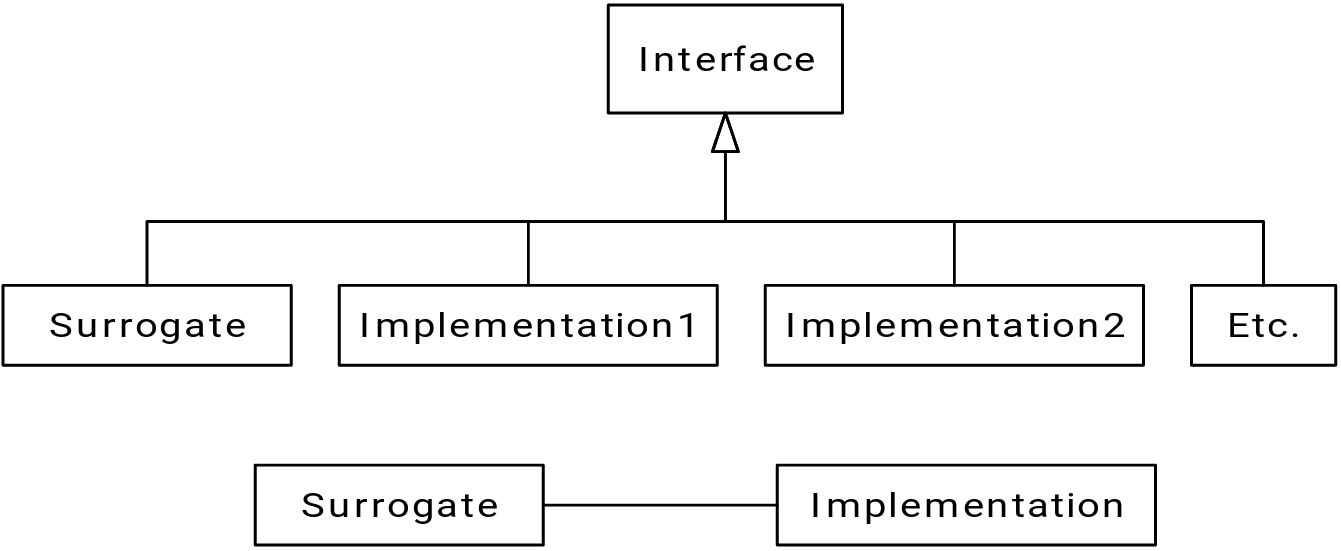
\includegraphics[width=\textwidth]{pg50} 
    \caption{tomado de: http://docs.linuxtone.org/ebooks/Python/Thinking\_In\_Python.pdf }
    \label{fig:mesh1}
\end{figure}

Cuando se crea un objeto sustituto, se da una implementación a la cual enviar todos los llamados a los métodos.    \newline

Estructuralmente, la diferencia entre \textit{Proxy} y \textit{State} es simple: un \textit{Proxy} tiene una sola implementación, mientras que \textit{State} tiene más de una implementación. La aplicación  de los patrones se considera en \textit{Design Patterns} (Patrones de Diseño) de forma distinta: \textit{Proxy} es usado para controlar el acceso a esta implementación, mientras \textit{State}  le permite cambiar la implementación de forma dinámica. Sin embargo, si expande su noción de "controlando el acceso a la implementación", entonces los dos encajan pulcramente juntos.

\subsection*{Proxy}
\label{subsec:Proxy}
\addcontentsline{toc}{subsection}{\nameref{subsec:Proxy}}

Si implementamos \textit{Proxy} siguiendo el diagrama anterior, se ve así:

 \begin{lstlisting} 
#: c04:ProxyDemo.py 
# Simple demonstration of the Proxy pattern. 

class Implementation: 
  def f(self):  
    print "Implementation.f()" 
  def g(self):  
    print "Implementation.g()"  
  def h(self):  
    print "Implementation.h()" 
    
class Proxy: 
  def __init__(self):  
    self.__implementation = Implementation()  
  # Pass method calls to the implementation: 
    def f(self): self.__implementation.f()  
  def g(self): self.__implementation.g()  
  def h(self): self.__implementation.h()  
  
p = Proxy() 
p.f(); p.g(); p.h() 
#:~ 
 \end{lstlisting}
 
No es necesario que \textbf{Implementation} tenga la misma interfaz que \textbf{Proxy}; siempre y cuando \textbf{Proxy} es de alguna manera \textit{ "speaking for"} ("hablando en nombre de") la clase se refiere a la llamada del método, para entonces la idea básica está satisfecha (tenga en cuenta que esta declaración está en contradicción con la definición de Proxy en GoF). Sin embargo, es conveniente tener una interfaz común para que \textbf{Implementation} se vea obligado a cumplir con todos los métodos que \textbf{Proxy} necesita llamar. \newline
	
Por supuesto, en Python tenemos un mecanismo de delegación integrado, lo que hace que el \textbf{Proxy} sea aún más simple de implementar:   \newline

\begin{lstlisting} 
#: c04:ProxyDemo2.py 
# Simple demonstration of the Proxy pattern. 

class Implementation2: 
  def f(self):  
    print "Implementation.f()" 
  def g(self):  
    print "Implementation.g()"  
  def h(self):  
    print "Implementation.h()" 
    
class Proxy2: 
  def __init__(self):  
    self.__implementation = Implementation2()  
  def __getattr__(self, name): 
    return getattr(self.__implementation, name) 
    
p = Proxy2() 
p.f(); p.g(); p.h(); 
#:~ 
\end{lstlisting}

La belleza de la utilización de  \textbf{\_\_getattr\_\_( )} es que \textbf{Proxy2} es completamente genérico, y no vinculada a cualquier implementación particular (en Java, un "proxy dinámico" bastante complicado ha sido creado para lograr esto mismo). 

\newpage

\subsection*{State}
\label{subsec:State}
\addcontentsline{toc}{subsection}{\nameref{subsec:State}}

El patrón \textit{State} añade más implementaciones a \textit{Proxy}, junto con una manera de cambiar de una implementación a otra durante tiempo de vida del sustituto: \newline

\begin{lstlisting} 
#: c04:StateDemo.py 
# Simple demonstration of the State pattern.

class State_d: 
  def __init__(self, imp):  
    self.__implementation = imp  
  def changeImp(self, newImp): 
    self.__implementation = newImp 
  # Delegate calls to the implementation: 
  def __getattr__(self, name): 
    return getattr(self.__implementation, name) 
    
class Implementation1: 
  def f(self):  
    print "Fiddle de dum, Fiddle de dee,"  
  def g(self):  
    print "Eric the half a bee."  
  def h(self):  
    print "Ho ho ho, tee hee hee,"  
    
class Implementation2: 
    def f(self):  
    print "We're Knights of the Round Table."  
  def g(self):  
    print "We dance whene'er we're able."  
  def h(self):  
    print "We do routines and chorus scenes"  
    
def run(b): 
  b.f() 
  b.g() 
  b.h() 
  b.g() 
  
b = State_d(Implementation1()) 
run(b) 
b.changeImp(Implementation2()) 
run(b) 
#:~ 
\end{lstlisting}

Se puede ver que la primera implementación se usa para una parte, a continuación, la segunda implementación se intercambia y se utiliza.     \newline

La diferencia entre \textit{Proxy} y \textit{State} está en los problemas que se resuelven. Los usos comunes para \textit{Proxy} como se describe en \textit{Design Patterns} son:

\begin{enumerate}[1.]

    \item \textbf{Proxy remoto.} Este proxy para un objeto en un espacio de dirección diferente. Se crea un proxy remoto de forma automática por el compilador RMI \textbf{rmic} ya que crea ramales y esqueletos.
    
    \item \textbf{Proxy virtual.} Esto proporciona "inicialización relajada" para crear objetos costosos por demanda.
    
    \item \textbf{Proxy de Protección.} Se usa cuando no se desea que el programador cliente tenga acceso completo a los objetos proxy.
    
    \item \textbf{Referencia inteligente.} Para agregar acciones adicionales cuando se accede al objeto proxy. Por ejemplo, o para llevar un registro del número de referencias que se realizan para un objeto en particular, con el fin de implementar el lenguaje \textit{copy-on-write} (copiar en escritura) y prevenir objeto aliasing.
    %Objeto aliasing   {sugerencias: objetos espejos}
    Un ejemplo sencillo es hacer el seguimiento del número de llamadas a un método en particular.
\end{enumerate}

Usted podría mirar una referencia de Python como un tipo de proxy de protección, ya que controla el acceso al objeto real de los demás (y asegura, por ejemplo, que no utilice una referencia nula). \newline

[[\textit{Proxy} y \textit{State} no son vistos como relacionados entre sí porque los dos se les da (lo que considero arbitrario) diferentes estructuras.
\textit{State}, en particular, utiliza una jerarquía de implementación separada pero esto me parece innecesario a menos que usted haya decidido que la implementación no está bajo su control (ciertamente una posibilidad, pero si usted es dueño de todo el código no parece haber ninguna razón para no beneficiarse de la elegancia y amabilidad de la clase base individual). En adición, \textit{Proxy} no necesita utilizar la misma clase base para su implementación, siempre y cuando el objeto proxy esté controlando el acceso al objetarlo "frente" a favor. %Corregir! 
Independientemente de los detalles, en ambos \textit{Proxy} y \textit{State} un sustituto está pasando la llamada al método a través de un objeto de implementación.]]

\newpage

\subsection*{StateMachine (Máquina de Estados)}
\label{subsec:sm}
\addcontentsline{toc}{subsection}{\nameref{subsec:sm}}


Mientras \textit{State} tiene una manera de permitir que el programador cliente cambie la implementación, \textit{StateMachine} impone una estructura para cambiar automáticamente la implementación de un objeto al siguiente. La implementación actual representa el estado en que un sistema está, y el sistema se comporta de manera diferente de un estado a otro (ya que utiliza \textit{State}). Basicamente, esta es una "state machine : máquina de estados" usando objetos.     \newline

El código que mueve el sistema de un estado a otro es a menudo un \textit{Template Method} (Método Plantilla), como se ve en el siguiente framework para una máquina de estados básica.    \newline

Cada estado puede estar en un \textbf{run( )} para cumplir con su comportamiento, y (en este diseño) también puede pasarlo a un objeto "input" y así puede decirle a que nuevo estado es removido basado en este "input".
La distinción clave entre este diseño y el siguiente es que aquí, cada objeto \textbf{State} decide lo que otros estados pueden avanzar, basado en "input”, mientras que en el posterior diseño de todas las transiciones de estado se llevan a cabo en una sola tabla. Otra forma de decirlo es que aquí, cada objeto \textbf{State} tiene su propia pequeña tabla \textbf{State}, y en el subsiguiente diseño hay una sola tabla directora de transición de estado para todo el sistema.   \newline

 \begin{lstlisting}
#: c04:statemachine:State.py 
# A State has an operation, and can be moved 
# into the next State given an Input: 

class State: 
  def run(self):  
    assert 1, "run not implemented" 
  def next(self, input): 
    assert 1, "next not implemented" 
#:~ 
 \end{lstlisting}
 
 Esta clase es claramente innecesaria, pero que nos permite decir que algo es un objeto \textbf{State} en el código, y proporcionar un mensaje de error ligeramente diferente cuando no se implementan todos los métodos. Podríamos haber conseguido básicamente el mismo efecto diciendo:      \newline
 
 \begin{lstlisting}
 class State: pass
 \end{lstlisting}
 
 Porque todavía conseguiríamos excepciones si \textbf{run} o \textbf{next()} hubieran sido llamados por un tipo derivado, y no hubieran sido implementados. \newline
 
El \textbf{StateMachine} hace un seguimiento de la situación actual, el cual es inicializado por el constructor. El método \textbf{runAll()} toma una lista de objetos \textbf{Input}. Este método no sólo avanza al siguiente estado, sino que también llama \textbf{run( )} para cada objeto \textit{state} – por lo tanto se puede ver que es una expansión de la idea del patrón \textbf{State}, ya que \textbf{run( )} hace algo diferente dependiendo del estado en que el sistema está.    \newline

\begin{lstlisting}
#: c04:statemachine:StateMachine.py 
# Takes a list of Inputs to move from State to  
# State using a template method. 

class StateMachine: 
  def __init__(self, initialState): 
    self.currentState = initialState 
    self.currentState.run() 
  # Template method: 
  def runAll(self, inputs): 
    for i in inputs: 
      print i 
      self.currentState = self.currentState.next(i) 
      self.currentState.run() 
#:~ 
\end{lstlisting}

También he tratado \textbf{runAll( )} como un método plantilla. Esto es típico, pero ciertamente no es necesario – posiblemente podría querer
%concievably == posiblemente
reemplazarlo, pero por lo general el cambio de comportamiento se producirá en \textbf{run( )} de \textbf{State} en su lugar.       \newline

En este punto se ha completado el framework básico para este estilo de StateMachine (donde cada estado decide los próximos estados). Como ejemplo, voy a utilizar una trampa de fantasía para que el ratón pueda moverse a través de varios estados en el proceso de atrapar un ratón\footnote{Ningún ratón fue perjudicado en la creación de este ejemplo.}. Las clases ratón y la información se almacenan en el paquete \textbf{mouse}, incluyendo una clase en representación de todas los posibles movimientos que un ratón puede hacer, que serán las entradas a la \textit{state machine} (máquina de estados):       \newline
% harm == dañar, perjudicar

\begin{lstlisting}
#: c04:mouse:MouseAction.py 

class MouseAction: 
  def __init__(self, action):  
    self.action = action 
  def __str__(self): return self.action  
  def __cmp__(self, other): 
    return cmp(self.action, other.action) 
  # Necessary when __cmp__ or __eq__ is defined 
  # in order to make this class usable as a 
  # dictionary key: 
  def __hash__(self):  
    return hash(self.action) 
    
# Static fields; an enumeration of instances: 
MouseAction.appears = MouseAction("mouse appears") 
MouseAction.runsAway = MouseAction("mouse runs away") 
MouseAction.enters = MouseAction("mouse enters trap") 
MouseAction.escapes = MouseAction("mouse escapes") 
MouseAction.trapped = MouseAction("mouse trapped") 
MouseAction.removed = MouseAction("mouse removed") 
#:~   
  \end{lstlisting}
  
Usted observará que \textbf{\_\_cmp\_\_( )} se ha reemplazado para implementar una comparación entre los valores de \textit{action}. También, cada posible movida de un ratón se enumera como un objeto de \textbf{MouseAction}, todos los cuales son los campos estáticos en \textbf{MouseAction}. \newline

Para la creación de código de prueba, una secuencia de entradas de mouse está provisto de un archivo de texto:  \newline
  
\begin{lstlisting}  
#:! c04:mouse:MouseMoves.txt 
mouse appears 
mouse runs away 
mouse appears 
mouse enters trap 
mouse escapes 
mouse appears 
mouse enters trap 
mouse trapped 
mouse removed 
mouse appears 
mouse runs away 
mouse appears 
mouse enters trap 
mouse trapped 
mouse removed 
#:~ 
\end{lstlisting}
 
 Con estas herramientas en su lugar, ahora es posible crear la primera versión del programa mousetrap (ratonera). Cada subclase \textbf{State} define su comportamiento \textbf{run( )} y también establece su siguiente estado con una sentencia \textbf{if-else}:   \newline
   
\begin{lstlisting}  
 #: c04:mousetrap1:MouseTrapTest.py 
# State Machine pattern using 'if' statements 
# to determine the next state. 
import string, sys 
sys.path += ['../statemachine', '../mouse'] 
from State import State 
from StateMachine import StateMachine 
from MouseAction import MouseAction 
# A different subclass for each state:

class Waiting(State): 
  def run(self):  
    print "Waiting: Broadcasting cheese smell" 
    
  def next(self, input): 
    if input == MouseAction.appears: 
      return MouseTrap.luring 
    return MouseTrap.waiting 
    
class Luring(State): 
  def run(self): 
    print "Luring:Presenting Cheese, door open" 
  def next(self, input): 
    if input == MouseAction.runsAway: 
      return MouseTrap.waiting 
    if input == MouseAction.enters: 
      return MouseTrap.trapping 
    return MouseTrap.luring 
    
class Trapping(State): 
  def run(self): 
    print "Trapping: Closing door"
    
  def next(self, input): 
    if input == MouseAction.escapes: 
      return MouseTrap.waiting 
    if input == MouseAction.trapped: 
      return MouseTrap.holding 
    return MouseTrap.trapping 
    
class Holding(State): 
  def run(self): 
    print "Holding: Mouse caught" 
   def next(self, input): 
    if input == MouseAction.removed: 
      return MouseTrap.waiting 
    return MouseTrap.holding 
    
class MouseTrap(StateMachine): 
  def __init__(self):  
    # Initial state 
    StateMachine.__init__(self, MouseTrap.waiting) 
    
# Static variable initialization: 
MouseTrap.waiting = Waiting() 
MouseTrap.luring = Luring() 
MouseTrap.trapping = Trapping() 
MouseTrap.holding = Holding() 

moves = map(string.strip,  
  open("../mouse/MouseMoves.txt").readlines()) 
MouseTrap().runAll(map(MouseAction, moves)) 
#:~ 
  \end{lstlisting}
  
  La clase \textbf{StateMachine} simplemente define todos los posibles estados como objetos estáticos, y también establece el estado inicial. \textbf{UnitTest} crea un \textbf{MouseTrap} y luego prueba con todas las entradas de un \textbf{MouseMoveList.}    \newline
  
  Mientras el uso de las sentencias \textbf{if} dentro de los métodos \textbf{next()} es perfectamente razonable, la gestión de un gran número de ellos podría llegar a ser difícil. Otro enfoque es crear tablas dentro de cada objeto \textbf{State} definiendo los diversos estados próximos basados en la entrada.    \newline
  
  Inicialmente, esto parece que debería ser bastante simple. Usted debe ser capaz de definir una tabla estática en cada subclase \textbf{State} que define las transiciones en términos de los otros objetos \textbf{State}. Sin embargo, resulta que este enfoque genera dependencias de inicialización cíclicas. Para resolver el problema, He tenido que retrasar la inicialización de las tablas hasta la primera vez que se llama al método  \textbf{next( )} para un objeto en particular \textbf{State}. Inicialmente, los métodos \textbf{next()} pueden parecer un poco extraños debido a esto.\newline
  
  La clase \textbf{StateT} es una implementación de \textbf{State} ((de modo que la misma clase \textbf{StateMachine} puede ser utilizado en el ejemplo anterior) que añade un \textbf{Map} y un método para inicializar el mapa a partir de una matriz de dos dimensiones. El "método \textbf{next()}" tiene una implementación de la clase base que debe ser llamado desde el "método \textbf{next()} de la clase derivada anulada", después de que se ponen a prueba para un \textbf{null Map} (y inicializarlo si es nulo):  \newline
  
 \begin{lstlisting}
#: c04:mousetrap2:MouseTrap2Test.py 
# A better mousetrap using tables 
import string, sys 
sys.path += ['../statemachine', '../mouse'] 
from State import State 
from StateMachine import StateMachine 
from MouseAction import MouseAction 

class StateT(State): 
  def __init__(self): 
    self.transitions = None 
  def next(self, input): 
    if self.transitions.has_key(input): 
      return self.transitions[input] 
    else: 
      raise "Input not supported for current state" 
class Waiting(StateT): 
  def run(self):  
    print "Waiting: Broadcasting cheese smell" 
  def next(self, input): 
    # Lazy initialization: 
    if not self.transitions: 
      self.transitions = {  
        MouseAction.appears : MouseTrap.luring  
      } 
    return StateT.next(self, input) 
class Luring(StateT): 
  def run(self): 
    print "Luring: Presenting Cheese, door open" 
  def next(self, input): 
    # Lazy initialization: 
    if not self.transitions: 
      self.transitions = { 
        MouseAction.enters : MouseTrap.trapping, 
        MouseAction.runsAway : MouseTrap.waiting 
      } 
    return StateT.next(self, input) 
class Trapping(StateT): 
  def run(self): 
  
      print "Trapping: Closing door" 
  def next(self, input): 
    # Lazy initialization: 
    if not self.transitions: 
      self.transitions = { 
        MouseAction.escapes : MouseTrap.waiting, 
        MouseAction.trapped : MouseTrap.holding 
      } 
    return StateT.next(self, input) 
class Holding(StateT): 
  def run(self): 
    print "Holding: Mouse caught" 
  def next(self, input): 
    # Lazy initialization: 
    if not self.transitions: 
      self.transitions = { 
        MouseAction.removed : MouseTrap.waiting 
      } 
    return StateT.next(self, input) 
class MouseTrap(StateMachine): 
  def __init__(self):  
    # Initial state 
    StateMachine.__init__(self, MouseTrap.waiting) 
# Static variable initialization: 
MouseTrap.waiting = Waiting() 
MouseTrap.luring = Luring() 
MouseTrap.trapping = Trapping() 
MouseTrap.holding = Holding() 
moves = map(string.strip,  
  open("../mouse/MouseMoves.txt").readlines()) 
mouseMoves = map(MouseAction, moves) 
MouseTrap().runAll(mouseMoves) 
#:~ 
 \end{lstlisting}
 
El resto del código es idéntico – la diferencia está en los métodos \textbf{next()} y la clase \textbf{StateT}.\newline

Si usted tiene que crear y mantener una gran cantidad de clases \textbf{State}, este enfoque es una mejora, ya que es más fácil de leer de forma rápida y comprender las transiciones de estado viendo la tabla.

\newpage

\subsection*{Table-Driven State Machine}
\label{subsec:tdsm}
\addcontentsline{toc}{subsection}{\nameref{subsec:tdsm}}

La ventaja del diseño anterior es que toda la información acerca de un estado, incluyendo la información de transición del estado,  se encuentra dentro de la misma clase \textit{state}. Esto es generalmente un buen principio de diseño.    \newline

Sin embargo, en una \textit{state machine} (máquina de estados) pura, la máquina puede ser completamente representada por una única tabla de transición de estados. Esto tiene la ventaja de localizar toda la información sobre la máquina de estados en un solo lugar, lo que significa que usted puede con mayor facilidad crear y mantener la tabla basada en un diagrama de transición de estados clásica.      \newline 

El diagrama clásico de transición de estados utiliza un círculo para representar cada estado, y las líneas del \textit{state} señalando a todos los estados en que \textit{state} puede trasladarse. Cada línea de transición se anota con condiciones para la transición y una acción durante la transición. El siguiente es su aspecto: \newline

(Diagrama State Machine simple) \newline

Objetivos:

\begin{itemize}
    \item Traducción directa del diagrama de estado
    \item Vector del cambio: la representación del diagrama de estado
    \item Implementación razonable
    \item No hay exceso de estados (usted podría representar a cada cambio individual con un nuevo estado)
    \item La simplicidad y la flexibilidad
\end{itemize}

Observaciones:

\begin{itemize}
    \item Los estados son triviales – ninguna información o funciones / datos, sólo una identidad.
    \item Diferente a \textit{State Pattern}!
    \item La máquina regula el paso de un estado a otro.
    \item Al igual que en flyweight : peso mosca
    \item Cada estado puede pasar a muchos otros
    \item Funciones de condición / acción también deben ser externos a los estados
    \item Centralizar la descripción en una sola tabla que contiene todas las variaciones, para facilitar la configuración.
\end{itemize}

Ejemplo:

\begin{itemize}
    \item State Machine y Table-Driven Code 
    \item Implementa una máquina expendedora
    \item Utiliza diferentes patrones
    \item Separa código común \textit{state-machine} de aplicaciones específicas (como método de plantilla)
    \item Cada entrada causa una búsqueda de la solución apropiada (como cadena de responsabilidad)
    \item Las pruebas y transiciones se encapsulan en objetos de funciones (objetos que contienen funciones)
    \item Restricción de Java: los métodos no son objetos de primera clase.
\end{itemize}

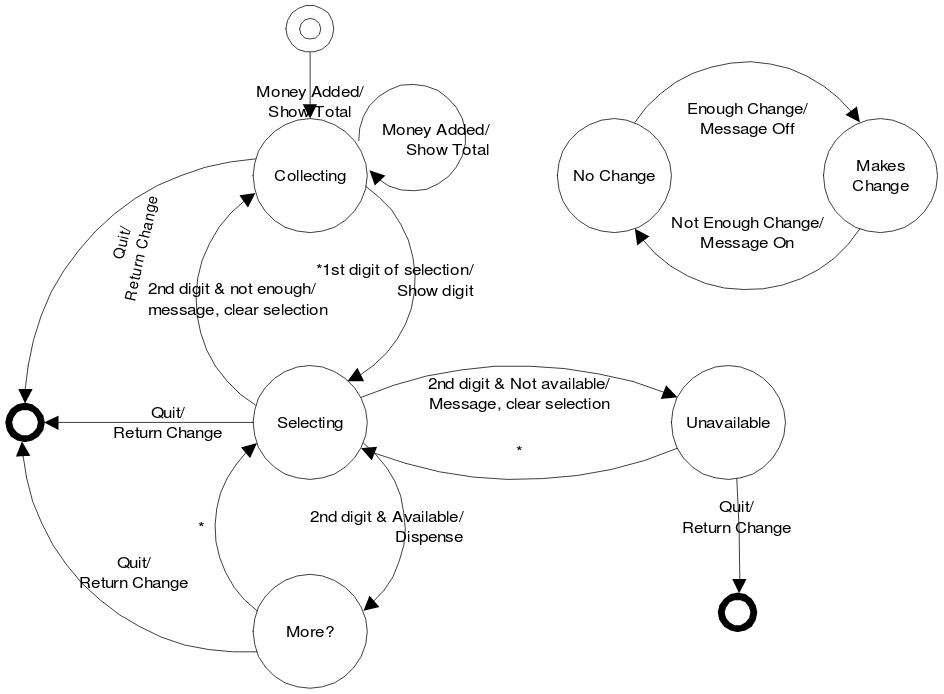
\includegraphics[width=\textwidth]{pag63}  


\subsubsection*{La clase State}
\label{subsubsec:lcs}
\addcontentsline{toc}{subsubsection}{\nameref{subsubsec:lcs}}

 La clase \textbf{State} es claramente diferente a la anterior, ya que es en realidad sólo un marcador de posición con un nombre. Por lo tanto, no se hereda de las clases \textbf{State} anteriores:    \newline
 
 \begin{lstlisting}
# c04:statemachine2:State.py 
class State: 
  def __init__(self, name): self.name = name 
  def __str__(self): return self.name  
# :~  
 \end{lstlisting}
  
  
\subsubsection*{Condiciones para la transición}
\label{subsubsec:cplt}
\addcontentsline{toc}{subsubsection}{\nameref{subsubsec:cplt}}  

En el diagrama de transición de estados, una entrada se pone a prueba para ver si satisface las condiciones necesarias para transferir al Estado en cuestión. Como antes, el \textbf{Input} es sólo una interfaz de etiquetado:     \newline

\begin{lstlisting}
# c04:statemachine2:Input.py 
# Inputs to a state machine 
class Input: pass 
# :~ 
\end{lstlisting}

La \textbf{Condition} evalúa el \textbf{Input} para decidir si esta fila en la tabla es la transición correcta: \newline

  \begin{lstlisting}
# c04:statemachine2:Condition.py 
# Condition function object for state machine 

class Condition: 
  boolean condition(input) :  
    assert 1, "condition() not implemented" 
# :~ 
\end{lstlisting}

\subsubsection*{Acciones de transición}
\label{subsubsec:adt}
\addcontentsline{toc}{subsubsection}{\nameref{subsubsec:adt}}


Si \textbf{Condition} devuelve \textbf{true}, entonces se hace la transición a un nuevo estado, y dado que esa transición se hace, algún tipo de acción ocurre (en el diseño anterior de \textit{state machine : máquina de estado}, éste era el método\textbf{run( )}).     \newline

\begin{lstlisting}
# c04:statemachine2:Transition.py 
# Transition function object for state machine 

class Transition: 
  def transition(self, input): 
    assert 1, "transition() not implemented" 
# :~ 
\end{lstlisting}

\subsubsection*{La tabla}
\label{subsubsec:lt}
\addcontentsline{toc}{subsubsection}{\nameref{subsubsec:lt}}

Con estas clases en el lugar, podemos establecer una tabla de 3 dimensiones, donde cada fila describe completamente un estado. El primer elemento en la fila es el estado actual, y el resto de los elementos de la fila, son los diferentes tipos de entradas posibles, la condición que se debe satisfacer para que este cambio de estado sea el correcto, la acción que ocurre durante la transición, y el nuevo estado al que se moverá dentro. Observe que el objeto \textbf{Input} no sólo se utiliza para su tipo, también es un objeto \textit{Messenger} que lleva la información a los objetos \textbf{Condition} y \textbf{ Transition} :     \newline

\begin{lstlisting}
{(CurrentState, InputA) : (ConditionA, TransitionA, NextA), 
 (CurrentState, InputB) : (ConditionB, TransitionB, NextB), 
 (CurrentState, InputC) : (ConditionC, TransitionC, NextC), 
 ... 
 }
\end{lstlisting}


\subsubsection*{La máquina básica}
\label{subsubsec:lmb}
\addcontentsline{toc}{subsubsection}{\nameref{subsubsec:lmb}}

\begin{lstlisting}
# c04:statemachine2:StateMachine.py 
# A table-driven state machine 

class StateMachine: 
  def __init__(self, initialState, tranTable): 
    self.state = initialState 
    self.transitionTable = tranTable 
    
  def nextState(self, input): 
  
    Iterator it=((List)map.get(state)).iterator() 
    while(it.hasNext()): 
      Object[] tran = (Object[])it.next() 
      if(input == tran[0] ||  
         input.getClass() == tran[0]): 
        if(tran[1] != null): 
          Condition c = (Condition)tran[1] 
          if(!c.condition(input)) 
            continue #Failed test
            
        if(tran[2] != null) 
          ((Transition)tran[2]).transition(input) 
        state = (State)tran[3] 
        return 
        
    throw RuntimeException( 
      "Input not supported for current state") 
      
# :~ 
\end{lstlisting}

\subsubsection*{Simple máquina expendedora}
\label{subsubsec:sme}
\addcontentsline{toc}{subsubsection}{\nameref{subsubsec:sme}}

\begin{lstlisting}
# c04:vendingmachine:VendingMachine.py 
# Demonstrates use of StateMachine.py 
import sys 
sys.path += ['../statemachine2'] 
import StateMachine 

class State: 
  def __init__(self, name): self.name = name 
  def __str__(self): return self.name  
State.quiescent = State("Quiesecent") 
State.collecting = State("Collecting") 
State.selecting = State("Selecting") 
State.unavailable = State("Unavailable") 
State.wantMore = State("Want More?") 
State.noChange = State("Use Exact Change Only") 
State.makesChange = State("Machine makes change") 

class HasChange: 
  def __init__(self, name): self.name = name 
  def __str__(self): return self.name  
  
HasChange.yes = HasChange("Has change") 
HasChange.no = HasChange("Cannot make change") 

class ChangeAvailable(StateMachine): 
  def __init__(self): 
    StateMachine.__init__(State.makesChange, { 
      # Current state, input 
      (State.makesChange, HasChange.no) : 
        # test, transition, next state: 
        (null, null, State.noChange), 
      (State.noChange, HasChange.yes) : 
        (null,null, State.noChange) 
    }) 
    
class Money: 
  def __init__(self, name, value): 
    self.name = name 
    self.value = value 
  def __str__(self): return self.name  
  def getValue(self): return self.value 
  
Money.quarter = Money("Quarter", 25) 
Money.dollar = Money("Dollar", 100) 

class Quit: 
  def __str__(self): return "Quit"  
  
Quit.quit = Quit() 

class Digit: 
  def __init__(self, name, value): 
    self.name = name 
    self.value = value 
  def __str__(self): return self.name  
  def getValue(self): return self.value  
  
class FirstDigit(Digit): pass 
FirstDigit.A = FirstDigit("A", 0) 
FirstDigit.B = FirstDigit("B", 1) 
FirstDigit.C = FirstDigit("C", 2) 
FirstDigit.D = FirstDigit("D", 3) 

class SecondDigit(Digit): pass 
SecondDigit.one = SecondDigit("one", 0) 
SecondDigit.two = SecondDigit("two", 1) 
SecondDigit.three = SecondDigit("three", 2) 
SecondDigit.four = SecondDigit("four", 3) 

class ItemSlot: 
  id = 0 
  def __init__(self, price, quantity): 
    self.price = price 
    self.quantity = quantity 
  def __str__(self): return `ItemSlot.id` 
  def getPrice(self): return self.price  
  def getQuantity(self): return self.quantity  
  def decrQuantity(self): self.quantity -= 1 
  
class VendingMachine(StateMachine): 
  changeAvailable = ChangeAvailable() 
  amount = 0 
  FirstDigit first = null 
  ItemSlot[][] items = ItemSlot[4][4] 
  
  # Conditions: 
  def notEnough(self, input): 
    i1 = first.getValue() 
    i2 = input.getValue() 
    return items[i1][i2].getPrice() > amount 
    
  def itemAvailable(self, input): 
    i1 = first.getValue() 
    i2 = input.getValue() 
    return items[i1][i2].getQuantity() > 0 
    
  def itemNotAvailable(self, input): 
    return !itemAvailable.condition(input) 
    #i1 = first.getValue() 
    #i2 = input.getValue() 
    #return items[i1][i2].getQuantity() == 0 
    
  # Transitions: 
  def clearSelection(self, input): 
    i1 = first.getValue() 
    i2 = input.getValue() 
    ItemSlot is = items[i1][i2] 
    print ( 
      "Clearing selection: item " + is + 
      " costs " + is.getPrice() + 
      " and has quantity " + is.getQuantity()) 
    first = null 
    
  def dispense(self, input): 
    i1 = first.getValue() 
    i2 = input.getValue() 
    ItemSlot is = items[i1][i2] 
    print ("Dispensing item " +  
      is + " costs " + is.getPrice() + 
      " and has quantity " + is.getQuantity()) 
    items[i1][i2].decrQuantity() 
    print ("Quantity " +  
      is.getQuantity()) 
    amount -= is.getPrice() 
    print("Amount remaining " +  
      amount) 
      
  def showTotal(self, input): 
    amount += ((Money)input).getValue() 
    print "Total amount = " + amount 
    
  def returnChange(self, input): 
    print "Returning " + amount 
    amount = 0 
    
  def showDigit(self, input): 
    first = (FirstDigit)input 
    print "First Digit= "+ first 
    
    
      def __init__(self): 
    StateMachine.__init__(self, State.quiescent) 
    for(int i = 0 i < items.length i++) 
      for(int j = 0 j < items[i].length j++) 
        items[i][j] = ItemSlot((j+1)*25, 5) 
    items[3][0] = ItemSlot(25, 0) 
    buildTable(Object[][][]{ 
     ::State.quiescent, # Current state 
        # Input, test, transition, next state: 
       :Money.class, null,  
         showTotal, State.collecting, 
     ::State.collecting, # Current state 
        # Input, test, transition, next state: 
       :Quit.quit, null,  
         returnChange, State.quiescent, 
       :Money.class, null,  
         showTotal, State.collecting, 
       :FirstDigit.class, null,  
         showDigit, State.selecting, 
     ::State.selecting, # Current state 
        # Input, test, transition, next state: 
       :Quit.quit, null,  
         returnChange, State.quiescent, 
       :SecondDigit.class, notEnough,  
         clearSelection, State.collecting, 
       :SecondDigit.class, itemNotAvailable,  
         clearSelection, State.unavailable, 
       :SecondDigit.class, itemAvailable,  
         dispense, State.wantMore, 
     ::State.unavailable, # Current state 
        # Input, test, transition, next state: 
       :Quit.quit, null,  
         returnChange, State.quiescent, 
       :FirstDigit.class, null,  
         showDigit, State.selecting, 
     ::State.wantMore, # Current state 
        # Input, test, transition, next state: 
       :Quit.quit, null,  
         returnChange, State.quiescent, 
       :FirstDigit.class, null,  
         showDigit, State.selecting, 
    ) 
    # :~ 
\end{lstlisting}

\subsubsection*{Prueba de la máquina}
\label{subsubsec:pdlm}
\addcontentsline{toc}{subsubsection}{\nameref{subsubsec:pdlm}}


\begin{lstlisting} 
# c04:vendingmachine:VendingMachineTest.py 
# Demonstrates use of StateMachine.py 

vm = VendingMachine() 
for input in [   
    Money.quarter, 
    Money.quarter, 
    Money.dollar, 
    FirstDigit.A, 
    SecondDigit.two, 
    FirstDigit.A, 
    SecondDigit.two, 
    FirstDigit.C, 
    SecondDigit.three, 
    FirstDigit.D, 
    SecondDigit.one, 
    Quit.quit]: 
  vm.nextState(input) 
# :~ 
\end{lstlisting}


\subsection*{Herramientas}
\label{subsec:Herramientas}
\addcontentsline{toc}{subsection}{\nameref{subsec:Herramientas}}

Otro enfoque, ya que su \textit{state machine} (máquina de estado) se hace más grande, es el uso de una herramienta de automatización mediante el cual se configura una tabla y se deja que la herramienta genere el código state machine para usted. Esto puede ser creado por sí mismo utilizando un lenguaje como Python, pero también hay herramientas libres de código abierto como \textit{Libero}, en \url{http://www.imatix.com/} \newline 


\subsection*{Ejercicios}
\label{subsec:Ejercicios}
\addcontentsline{toc}{subsection}{\nameref{subsec:Ejercicios}}

1. Crear un ejemplo del "proxy virtual". \newline

2. Crear un ejemplo del proxy "Referencia Inteligente" donde se guarda la cuenta del número de llamadas a los métodos y a un objeto en particular. \newline

3. Crear un programa similar a ciertos sistemas DBMS (Sistema Manejador de Bases de Datos) que sólo permiten un cierto número de conexiones en cualquier momento. Para implementar esto, utilizar 'Singleton' como un sistema que controla el número de objetos "connections" que se crean. Cuando un usuario ha terminado con una conexión, el sistema debe ser informado de manera que pueda comprobar que la conexión volverá a ser reutilizada. Para garantizar esto, proporcionar un objeto proxy en lugar de una referencia a la conexión actual, y diseñar el proxy de manera que haga que la conexión a ser liberada regrese al sistema.   \newline

4. Usando \textit{State}, hacer una clase llamada \textbf{UnpredictablePerson} que cambia el tipo de respuesta a su método \textbf{hello( )} dependiendo de qué tipo de \textbf{Mood} está adentro. Añada un tipo de clase adicional \textbf{Mood} llamada \textbf{Prozac}.  \newline

5. Cree una copia simple en la implementación de escritura.   \newline

6. Aplicar \textbf{TransitionTable.py} al problema "Washer : Lavadora"  \newline

7. Crear un sistema \textit{StateMachine} mediante el cual el estado actual junto con la información de entrada determina el siguiente estado en que el sistema estará. Para hacer esto, cada estado debe almacenar una referencia de nuevo al objeto proxy (el controlador de estado) de modo que pueda solicitar el cambio de estado. Use un \textbf{HashMap} para crear una tabla de estados, donde la clave es un \textbf{String} que nombre el nuevo estado y el valor es el nuevo estado del objeto. Dentro de cada subclase \textbf{state} reemplazar un método \textbf{nextState( )} que tiene su propia tabla de transición de estados. La entrada a \textbf{nextState( )} debe ser una sola palabra que sale de un archivo de texto que contiene una palabra por línea.  \newline

8. Modificar el ejercicio anterior para que la \textbf{state machine} pueda ser configurada mediante la creación / modificación de una sola matriz multidimensional. \newline

9- Modificar el ejercicio  "mood” de la sesión anterior para que se convierta en una  \textbf{state machine} (máquina de estado) usando StateMachine.java     \newline

10. Crear un sistema elevador de \textbf{state machine} utilizando StateMachine.java     \newline

11. Crear un sistema de calefacción / aire acondicionado usando StateMachine.java   \newline

12. Un \textit{generator}(generador) es un objeto que produce otros objetos, al igual que una fábrica, excepto que la función generador no requiere ningún argumento. Cree un \textbf{MouseMoveGenerator} que produce acciones correctas \textbf{MouseMove} como salidas cada vez que la función generador es llamada (es decir, el mouse debe moverse en la secuencia apropiada, por lo que los movimientos posibles se basan en el movimiento anterior – esto es otra state machine). Agregue un método \textbf{iterator( )} para producir un iterador, pero este método debe tomar un argumento  \textbf{int} que especifica el número de movimientos a producir antes de \textbf{hasNext( )} que retorna \textbf{false}.
